Unlike conventional hardware designs which are often meticulously handcrafted
by experts, evolvable hardware applies genetic algorithms to
flexible hardware platforms to automatically explore the design space of potential
circuit solutions to specified hardware problems \cite{541893}.
The space of all possible circuit designs is huge. Currently no deterministic
search procedures perform well navigating through all possible solutions.
Despite some serious shortcomings the best performance so far in automated
hardware design has been through the application of genetic algorithms.
Currently this approach has only been successfully used on relatively
trivial problems, due to huge scaling issues. But where it has been used
the application of the
robust nondeterminism inherent in genetic algorithms to hardware design
has correctly autonomously developed application specific hardware.

The remainder of this chapter is dedicated to outlining the motivation of the
project and setting project objectives. Chapter~\ref{chap:technical} deals with
the existing literature and provides the technical understanding required for the
rest of this thesis. In Chapter~\ref{chap:execution}, the high level design choices
made during the project will be outlined, followed by a thorough description of
the implementation details. Chapter~\ref{chap:evaluation} focusses on evaluating
the project and includes all tests conducted throughout the project. Finally,
Chapter~\ref{chap:conclusion} contains the conclusion to this dissertation.

\section{Evolvable Hardware \label{s:ehw}}
Decades of evolvable hardware research has explored the application of genetic algorithms to
the domain of hardware design. Genetic algorithms come from the field of natural
computing and use Darwinian-inspired probabilistic procedure to improve a population
of candidate solutions'
performance given a fitness criteria via evolutionary pressure \cite{Goldberg:1989:GAS:534133}.
In the case of evolvable hardware,
each individual is a bitstring which can be mapped onto a circuit design
and the fitness criteria is rooted
in the circuit's ability to perform some predefined function.

The most common evolvable hardware arrangements
are built on Field Programmable Gate Arrays (FPGAs), these are immensely
flexible integrated circuits and constitute the substrate that the genetic
algorithm creates a solution within. Each member of the population
represents an FPGA configuration, and the individual's fitness is based on the
physical performance of the chip when configured to the individual's specification.

Conventional circuit design requires a huge amount of domain specific knowledge.
Applying machine learning to hardware design constitutes a potential
offloading of this information, allowing a user to define the success
criteria for a circuit and letting the machine autonomously construct a novel solution.
Thus far, there have been great successes deploying evolvable hardware in a few
narrow domains; creating
user-specific prosthetic hand controllers \cite{Kajitani1999AnEH},
image filters \cite{HybridFilter}, arbitrary logic circuits
\cite{Vasicek2011}, and even industrial robot controllers capable of fault recovery \cite{10.1007/3-540-61093-6_6}.

Current solutions are severely limited by scaling issues. As a problem
gets larger, a larger FPGA is required to tackle it, this results in the
search space exploding in size and crippling search times. Another factor
contributing to the scaling issue is that of test-case scaling. When evolving
a 1-bit binary adder circuit there are 4 test cases; 0 + 0, 0 + 1, 1 + 0, and
1 + 1. However, when you attempt 2-bit addition this becomes 16 test cases,
for 4-bit addition 256 individual sums have to be trailed to evaluate a
candidate solution.
The vast search space and rigorous evaluation step
are the main problems with scaling evolvable hardware beyond trivial problems.

One of the advantages of genetic algorithms is also one of their largest
weaknesses; they excel in generating strange and esoteric solutions.
These novel solutions sometimes
outperform their more conventional hand-designed counterparts,
but due to the seemingly arbitrary way key design decisions are made,
by a genetic algorithm, direct comparison to known solutions is difficult. This makes
learning from a genetic algorithm design hard, often we know that solutions
work well but know {\em how} it works well. Analysis of the resulting hardware
produced by an evolvable hardware project rarely
extend beyond an acknowledgement of functional correctness.

An example of one such strange design
(although outside the domain of circuit synthesis),
created with genetic algorithms,
comes from NASA. Where an evolutionary algorithm designed an, ironically
alien looking, antenna for use in space (Figure~\ref{fig:antenna})\cite{Antenna}, this antenna performed better
than any hand designed counterpart.

Unfortunately many applications of genetic algorithms are not as
successful as NASA's antenna.
It is uncommon that, by many design metrics, genetic algorithms produce results
better than the hand designed alternatives. However, conventional hand designed
circuitry requires
a huge amount of intuition from experienced designers as they balance
knowledge about the manufacture process, fault probabilities, power
consumption, among any number of other requirements. Any effort to automate
this must be seriously explored.

Despite being a relatively old field, and serious developments in genetic
algorithms (and machine learning in a wider sense), evolvable hardware has for
stagnated in recent years. In this project, exploration into how modern
genetic algorithm techniques can improve on an algorithm capable of designing solutions
to conventional hardware problems, such as simple binary arithmetic, will
be conducted.
It is also hoped that an exploration into the scaling issue will highlight
the largest contributor to this problem and potential mitigation
strategies.

\subsection{Field Programmable Gate Arrays \label{ss:FPGAs}}
Field Programmable Gate Arrays \cite{Kuon:2008:FAS:1454695.1454696}
are the backbone of the vast majority of evolutionary
hardware setups. They are a type of integrated circuit which can be
configured after manufacture to perform a variety of operations. Conventionally
an FPGA design is specified in a hardware design language and then compiled into a chip-specific bitfile.
This bitfile is uploaded to the device and configures the internal components
to perform the defined task.

The core functionality is built from a homogeneous mesh of
thousands of Configurable Logic Blocks (CLBs).
Each of these blocks takes input from their
neighbouring cells, has an internal binary function, and sends distinct outputs
to each of the neighbouring cells. The values sent to each output can be the
result of the internal function or a direct mapping from any of the inputs. The function,
the input(s) to the function
and the values sent to each output are completely configurable. Figure~\ref{fig:fpga}
demonstrates the internal structure of a CLB and how they can be arranged to form a simple FPGA.
Modern FPGAs also have a host of more complex features, such as expansive input/output,
wide data throughput, and look up tables.
Configurations are stored on-chip in ROM as a bitfile. This bitfile is usually generated
extrinsically \cite{10.1007/978-3-540-46239-2_5} and loaded onto the device \cite{Kuon:2008:FAS:1454695.1454696}.
If properly configured (and containing an appropriate number of CLBs) an FPGA can
functional identically to any printed digital circuit. They can be thought of
as the polar opposite to an ASIC (Application Specific Integrated Circuit), in that
rather than only performing one manufacturer-defined function, as ASICs do,
their functionality can be modified at will.
FPGAs share the power efficiency and execution proficiency of ASIC hardware, but
are considerably more expensive at scale.

When a great number of chips are required ASIC development makes sense; however, when a user needs
ASIC-like performance for only a handful of devices, it can often make more fiscal sense
to develop an FPGA configuration which matches the design needs.
This is because ASIC development can
be a lengthy and expensive process.
The limited number chips required and associated small-scale manufacturing
costs often makes FPGA development the clear option. This pressure for highly specific cost
effective hardware on a small scale
has driven mainstream FPGA development. One FPGA chip design can service many specific
hardware needs.

\begin{figure}
\centering
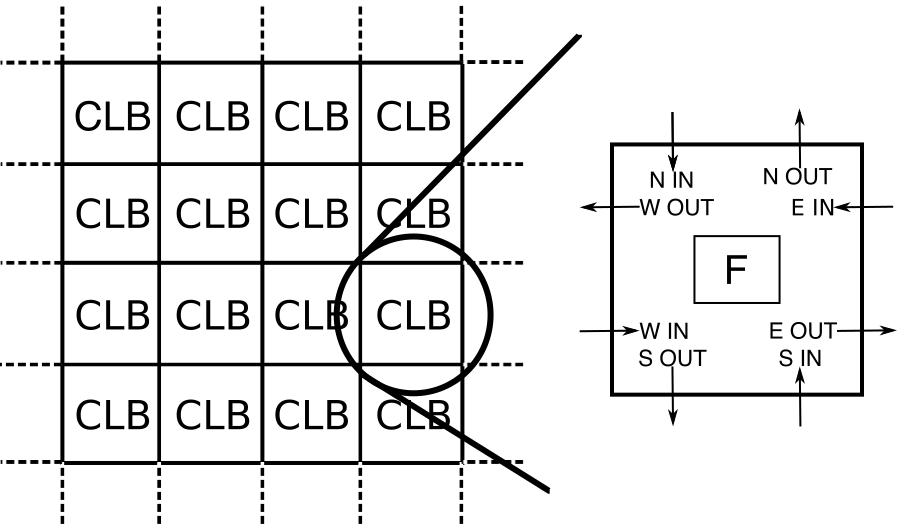
\includegraphics[width=.7\textwidth]{fpga.png}
\caption{FPGA architecture}
\label{fig:fpga}
\end{figure}

These immensely flexible circuits see wide use across industry. The most immediately
obvious example is
within firms developing more conventional integrated circuits who also ship accompanying
software. In these situations a team of engineers can develop software
while the hardware is developed in parallel, by using an FPGA loaded with a beta version
of chip. This avoids the many month wait times for a finished chip to be fabricated.
Recently FPGAs have seen a great deal of use as deep learning accelerators
\cite{Zhang:2015:OFA:2684746.2689060}; this is because FPGAs
configurations are cheaper to develop than ASIC hardware,
and see huge performance and power consumption benefits over more general purpose
hardware (GPGPUs for example). The flexibility also means iterative improvements
can be made to coincide with emerging research without the need to purchase new
hardware. Similarly, many industrial institutions require
bespoke hardware solutions to small-scale specific problems; suppose there is a
demand for a real time, high performance
pump controller which will only be used in a handful of locations. In these situations,
more often than not, ASIC
development is too expensive and not worth the narrow application setting. This demand has resulted in
the widespread use of FPGAs
in roles requiring an ASIC but without the market pressure to drive ASIC development
\cite{4267891}.
An application specific design can be built on an FPGA, while approaching peak performance and power
efficiency without massive development costs.
The military \cite{1346835} and aerospace \cite{henaut2009fpga} sectors use FPGAs extensively for these reasons along with
the built-in cryptographic and anti-tamper hardware obfuscation capabilities on
military-grade FPGAs.

\subsection{Genetic Algorithms}
The core of any genetic algorithm takes a randomly seeded population of binary strings
and applies
evolutionary pressure by performing a cycle of selection, crossover (an optional
step), and mutation
to move the population towards potential solutions to a given problem \cite{Goldberg:1989:GAS:534133}.
Beyond this there are many
variations, some of which will be explored in this thesis. The basic genetic algorithm is
outlined in Algorithm~\ref{alg:basic}.

\begin{algorithm}
	Randomly initialise a population $P$\\
	\While{evolving}{
		$Evaluate(P)$\\
		\While{New population $P'$ not full}{
			\eIf{Crossover occurs}{
				$p_1 \leftarrow Select(P)$\\
				$p_2 \leftarrow Select(P)$\\
				$i_1,i_2 \leftarrow Crossover(p_1,p_2)$\\
				Add $i_1$ and $i_2$ to $P'$
			}{
				$i \leftarrow Select(P)$\\
				Add $i$ to $P'$
			}
		}
		$P \leftarrow Mutate(P')$
	}
	\caption{Basic genetic algorithm}
	\label{alg:basic}
\end{algorithm}

An initial population is randomly generated and then
evaluated ($Evaluate(P)$). Evaluation provides each individual in the population with a score.
Members of a new population are generated by selecting members of the old population
at random, based on some selection mechanism (the most common schemes will be outlines
in Chapter~\ref{chap:technical}) and the scores each individual received. The individuals
selected in this manner have a single parent, some genetic algorithms also have a mechanism
by which an individual can have two parents; this is called crossover. Crossover has a
random chance of occurring, if it does, two individuals are selected from the old
population (via $Select(P)$), then from a random point in each parent's bitstring, the
parents swap
genetic material. This generates two new individuals, both are added to the
new population.
Finally, if an individual is made up of a bitstring of length $l$ and we have a mutation rate
of $m$, the $Mutate(P')$ function iterates over each bit in each individual, flipping the bit with
probability $\frac{m}{l}$. The new population $P'$ then replaces the old $P$, and the cycle continues.
These simple processes coalesce into a high performance robust search
procedure. Genetic algorithms are covered in more detail in Section~\ref{s:genetic}.

\subsection{Genetic Algorithms with an FPGA Configuration}
In a biology a genotype is an organism's DNA, and a phenotype is
the organism itself, the expression of the DNA. In the context of genetic algorithms,
the genotype is a binary string which is mapped onto a phenotype (in evolvable
hardware, often an FPGA configuration). When designing an evolvable hardware
system one must decide how to map from binary string to FPGA configuration.

Given a mapping from binary string to FPGA configuration and an FPGA test bed, one can
evaluate a population of bitstrings as the FPGA configuration to solve some digital
problem. This framework is at the core of evolutionary hardware. The bottleneck for physical evolvable
hardware is often the evaluation step, this involves converting each individual
to an FPGA configuration, uploading each in turn
to the FPGA, and extensively testing it. When each upload takes in the order of
multiple seconds the evaluation process can be laborious. To resolve this problem
many platforms simulate an FPGA until a design is chosen to be deployed, this reduces
training time aggressively, and is the direction this project has taken.

\section{Dynamic Problems}

A problem with evaluation critera which shifts over time is termed a dynamic problem.
Designing
evolutionary hardware robust to this set of problems is of considerable benefit as
dynamic problems span a class of practical but notoriously problematic challenges including
real-time optimisation, and fault tolerance.

\subsection{Hardware Faults}
Hardware faults are catastrophic for electronic devices. A relatively short life span is
mostly accepted, and is relatively benign in many areas; but when the cost of replacement is
extraordinarily high or the scale of the operation is large enough, there are huge benefits
to improving the fault tolerance of devices. An extreme example of the high cost of replacement
can be found with satellites, surveys of in-orbit satellites reveal that once deployed the
reliability of satalites drops aggressively, and despite the highest manufacturing standards,
after 15 years reliability drops to below
90\% \cite{CASTET20091718}. Be it due micrometeor impacts,
or the ionising effects of radiation, satellites are known to fail and a great deal of
work is expended improving their reliability. With the cost
of putting a satellite into orbit set in the millions of pounds, extending the lifespan
of such devices would have significant economic impact.

A little closer to home, data centres are vast structures contain thousands of servers.
Each of these has an 8\% probability of experiencing a failure each year
 \cite{Vishwanath:2010:CCC:1807128.1807161}.
Individually this is of no great concern, but when compounded across an entire data centre
server recovery and replacement becomes a primary concern for the management of
such an establishment.

One popular use of dynamic problems in evolutionary hardware is designed to breed
fault tolerance into a
design. This involves repeatedly turning on and off simulated faults in the FPGA during
evaluation in order to
create a design both robust to faults and not dependent on faults, as could happen if
only evaluated in a faulty system \cite{651463}. Another fault resilience
technique requires evaluating the configuration
against a fault-free FPGA and then combining the result with evaluation runs on FPGAs
simulating known frequent faults \cite{651463}\cite{Keymeulen2000}. These faults could include component
wear out, and manifest as blocked communications between CLBs or render the function
performed by a CLB inert. This extension of the fitness function (rather than
mid-execution fitness function modification) removes this approach from the domain of dynamic problems,
but it is worth noting as an alternate method to improve circuit reliability.

All of these methods require faults to be set before the genetic process begins, and can only be used to
develop evolvable hardware tolerant to specific faults. This requires a huge amount of knowledge
about the underlying hardware implementation and the frequency and severity of faults to generate
accurate fault models. This
is an important avenue of exploration but with evolvable hardware there is a missed
opportunity, with a system capable of quick iterative improvements, to work around
a problem as it occurs. This idea has been briefly explored in \cite{10.1007/3-540-61093-6_6}.

\subsection{Dynamic optimisation}
Another successful area of dynamic problems with evolutionary hardware involves
extending the evaluation function when a perfect solution has been found \cite{785435}. For example,
one could successfully evolve an audio filter and then incorporate a measure of ``smallness"
into the fitness. This would add evolutionary pressure to not only be correct, but also
use as little of the FPGA resources as possible.

Little work has been done exploring the reaction of evolvable hardware to tackling
related-but-not-identical problems (addition and subtraction, for example), and observing
the effect of varying
the relative benefits for correct answers for either, on the performance of the circuit for each problem.
Information in this domain could
drive development of systems capable of dynamically optimising in real-time
under shifting conditions.

\section{Project Aims}

The broad aim of this project is to develop an improved evolvable hardware
platform capable of effectively addressing dynamic problems. More specifically:
\begin{itemize}
	\item Apply the genetic algorithm from \cite{10.1007/3-540-63173-9_61} to
		the binary arithmetic problem.
	\item Combine state of the art genetic algorithms to improve
		evolvable hardware performance for binary arithmetic.
	\item Explore the application of evolvable hardware to dynamic
		problems, including FPGA faults and weighted binary arithmetic.
	\item Develop a specialised FPGA simulator to act as the evaluation
		back end for the genetic algorithm.
	\item Study and improve the scaling performance of evolvable hardware.
\end{itemize}

\section{Project Challenges}
The project is not without challenges:
\begin{itemize}
	\item There are few ways to evaluate individuals and population health beyond how
		correct they are, so understanding why a system works or does not work may
		be difficult.
	\item The issue of scaling will slow development of anything other than
		trivial problems (2-bit addition and subtraction).
	\item FPGA configurations for a variety of problems investigated here are very fragile, in the
		context of evolution. Frequent mutations could be disastrous.
	\item More so than in many evolutionary contexts the prospect of evolutionary dead ends
		and dominating local optima will need to be addressed.
\end{itemize}
